\section{Der Gradient}\label{chapter:00_gradient}
Der Gradient beschreibt einen Vektor, welcher in Richtung des steilsten Anstiegs einer Funktion zeigt.
Die Komponenten des Gradientenvektors bestehen aus den partiellen Ableitungen der Funktion an der jeweiligen Variablen.
\begin{align}
    \nabla f(x,y) \longrightarrow \begin{pmatrix} \frac{\delta f(x,y)}{\delta x} & \frac{\delta f(x,y)}{\delta y} \end{pmatrix}
\end{align}
Geometrisch kann dies an der Position $(x = 1, y = 1)$ für die Funktion $f(x, y) = x^2 + y^2$  wie in Abbildung
\ref{fig:01_gradient} aussehen. Zu beachten sei hier, dass der eigentliche Gradient in der XY-Ebene liegt (blau).
Der schwarze Vektor soll lediglich anzeigen, was eine Verschiebung in dieser Richtung bei der Eingabe der Variablen
für den Ausgabewert der Funktion bedeutet. Die Länge des Gradienten entspricht der Stärke der Steigung an diesem Punkt.

\begin{figure}[h!]
    \begin{center}
        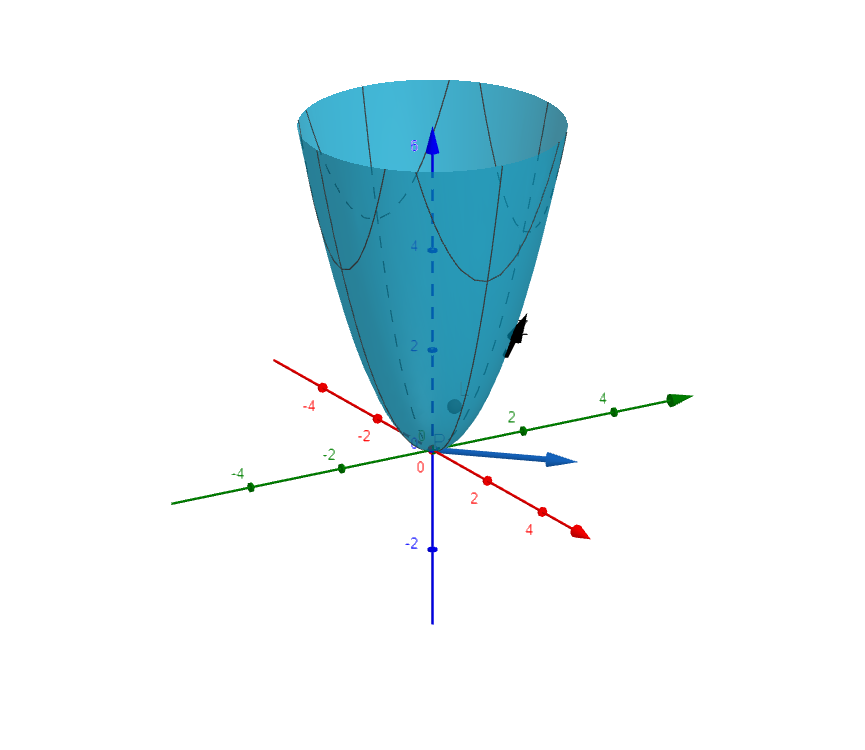
\includegraphics[width=0.6\linewidth]{../common/02_appendix/00_resources/01_gradient.png}
    \end{center}
    \caption{Gradient an der Position $(1, 1)$}
    \label{fig:01_gradient}
\end{figure}

\section{Das Gradientenabstiegsverfahren}\label{chapter:01_gradientenabstiegsverfahren}
Hierbei handelt es sich um ein Optimierungsverfahren, um einen Maximal- oder Minimalwert einer gegebenen Zielfunktion
zu finden. Es wird in dem Fall der Gradient, wie in Kapitel \ref{chapter:00_gradient} besprochen, verwendet. Die Idee
ist, dass man bei einer Maximierung in kleinen Schritten in Richtung des Gradienten folgt. Als Beispiel wird eine
Funktion angegeben, die von zwei Variablen $x, y$ abhängig ist. Beim Wert $\lambda$ handelt es sich um die Lernrate, welche
die Länge der zu gehenden Schritte beeinflusst. Der $\vec{\nabla}$ steht hierbei für den Gradienten.
\begin{align}
    \begin{pmatrix}x_{neu} & y_{neu}\end{pmatrix} = \begin{pmatrix}x_{alt} & y_{alt}\end{pmatrix} + \lambda \cdot \vec{\nabla}
\end{align}
Geometrisch kann wiederum die Abbildung \ref{fig:01_gradient} hinzugezogen werden. Dort würde man in einem ersten Schritt
in Richtung des schwarzen Vektors gehen, respektive in Richtung des Blauen, wenn man nur die Variablen beachtet.